% \documentclass[ukrainian,utf8,simple,floatsubsection, hpadding=5mm,equationsubsection,]{eskdtext}
% \usepackage[warn]{mathtext}
% \usepackage[unicode]{hyperref} % enable hyperlinks (активувати посилання)
% \usepackage{amssymb} % special math characters
% \usepackage{amsmath} % using cyrillic in formulae
% \usepackage{amsfonts} % special math fonts
% \usepackage{eskdtotal} 
% \usepackage{graphicx,epstopdf} % epstopdf-convert eps files to pdf
% \graphicspath{{algorithms/}{schemes/}{software/}{fig/}} % look up folders for figures
% \usepackage{listings} % to add source codes
% \usepackage{longtable} % multipage tables
% \usepackage{multirow} % using rowspan in tables
% \usepackage{nomencl} % support for abbreviations
% \makenomenclature % generate abbrevs index file
% \usepackage{float}
% % variables.tex
% This file contains information about author and other specific
% people for use in eskdx collection.

\title{\fontsize{12}{12} \selectfont Інтегрована інерціально-супутникова система навігації, що базується на принципах комплексної обробки інформації
з використанням калманівської фільтрації}
% smaller size of font set for the title in frame
\author{НовікМ.В.}

\ESKDchecker{ФіляшкінМ.К.}
\ESKDnormContr{КозловА.П.}
\ESKDapprovedBy{СинєглазовВ.М.}

\ESKDdepartment{Міністерство освіти і науки України}
\ESKDcompany{Національний авіаційний університет}

\ESKDsignature{НАУ 11 09 02 000 ПЗ}
\ESKDgroup{ІАСУ 608}

\ESKDsectAlign{section}{Center}
\ESKDsectAlign{subsection}{Center}
\ESKDsectAlign{subsubsection}{Center}

 % class parameters tuning
% \ESKDcolumnXIfIV{РусаловськийА.В.}
% \ESKDstyle{formIIab}
% \renewcommand\labelenumi{\arabic{enumi}.} 
% \renewcommand\labelenumii{\theenumi.\arabic{enumii}.}
% \renewcommand\labelenumiii{\arabic{enumi}.\arabic{enumii}.\arabic{enumiii}.}
% \begin{document}
% \ESKDthisStyle{formII}
\section{Охорона праці}
\subsection{Вступ}

В дипломній роботі розробляється інерціально-супутникова навігаційна система, що базується на основі комплексної обробки інформації з використанням фільтра Калмана. Розробкою та відпрацюванням алгоритмів роботи навігаційної системи, налаштуванням обладнання та калібровкою датчиків займаються інженери програмісти та радіотехніки лабораторії. Отже суб’єктом є інженер програміст лабораторії, функціональним зобов'язаннями якого є програмування навігаційних алгоритмів для бортової обчислюваної машині, засобом праці є персональний комп'ютер та модулі навігаційного обладнання: датчики навігаційної системи (мікромеханічні чи лазерні акселерометри та гіроскопи), бортовий обчислювач навігаційної інформації.

До роботи з навігаційним обладнанням та ЕОМ допускаються працівники, що не мають медичних протипоказань, пройшли вчасно періодичний медичний огляд, інструктаж і навчання  правилам техніки безпеки і виробничої санітарії.

Основним місцем роботи інженера програміста є лабораторія навігаційного обладнання авіаційного підприємства чи науково-дослідного інституту. Періодично місцем роботи може бути літак, де встановлено навігаційне обладнання (налаштування, тестування, випробування) або ЗПС, у випадку, якщо розроблені пристрої встановлюються на БПЛА.

\subsection{Опис робочого місця}
Для приміщення лабораторії вибрана площа 30 $\text{м}^2$, з висотою стелі -- 3м. Виробничі будівлі та приміщення споруджуються згідно з вимогами будівельних і санітарних норм. Об’єм виробничих приміщень для програмістів, операторів відеотермінальних пристроїв на одного працівника складає 19,5 $\text{м}^2$, площа приміщень — 6 м2 з урахуванням максимального числа працівників в одну зміну. 

\begin{figure}[H]
\centering
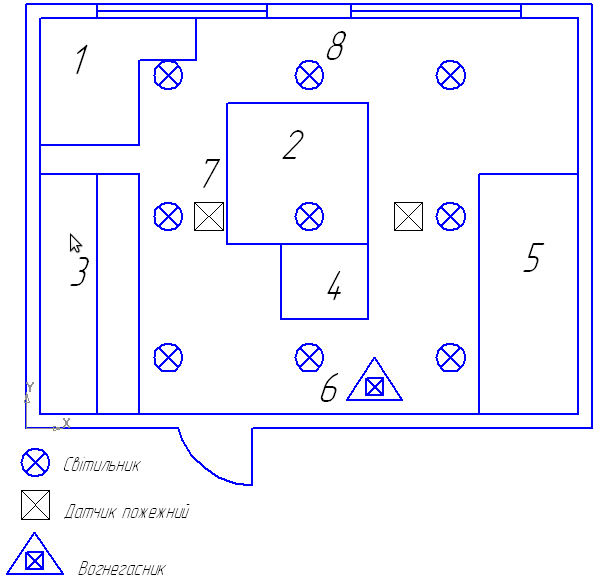
\includegraphics[scale=0.5]{lab_plan}
\caption{План робочого приміщення}\label{fig:lab_plan}
\end{figure}

\begin{enumerate}
 \item Робоче місце №1;
 \item Координатна платформа;
 \item Робоче місце №2;
 \item Стіл з ПК приєднаний до мережі та до вимірювальної апаратури;
 \item Шафа з допоміжним обладнанням та витратними матеріалами;
 \item Вогнегасник;
 \item Датчик пожежний;
 \item Світильник.
\end{enumerate}

В приміщенні розташовані два робочих місця. Перше обладнане ПК з рідкокристалічним дисплеєм, приєднане до локальної мережі. На столі додатково встановлені програматори, осцилограф, лабораторний блок живлення та мультиметр, телефон, принтер. Друге робоче місце обладнане паяльною станцією, контрольно-вимірною апаратурою, лабораторним блоком живлення, та додатковими розетками з мережею живлення 115В 400Гц. ПК, приєднаний до локальної мережі Ethernet. Над столом знаходиться полиця з радіоелементами. Всі прилади мають бути заземлені.

Трудова діяльність інженера програміста відбувається у певному виробничому середовищі, де діють такі шкідливі фактори: 
\begin{enumerate}
  \item Понижений рівень штучного освітлення 
  \item Шум
  \item Електричний струм
  \item Пожежонебезпека
  \item Мікроклімат

\end{enumerate}

\subsection{Шум}

Допустимі рівні звукового тиску у октавних смугах частот, еквівалентні рівні звуку на робочому місці регламентовані ДСН 3.3.6.037-99, для інженера показані в таблиці \ref{tb:noise}.
\begin{table}[H]
\small
\caption{Нормовані рівні звукового тиску та рівень шуму на робочому місці}
\centering
\begin{tabular}{|p{0.4in}|p{0.4in}|p{0.4in}|p{0.4in}|p{0.4in}|p{0.4in}|p{0.4in}|p{0.4in}|p{0.4in}|p{0.4in}|} \hline 
\multicolumn{9}{|p{4in}|}{Рівні звукового тиску (дБ) в  октавних смугах з серединами геометричними частотами, Гц} & Рівень звуку, дБА \\ \hline 
31.5 & 63 & 125 & 250 & 500 & 1000 & 2000 & 4000 & 8000 & 50 \\ \hline 
86 & 71 & 61 & 54 & 49 & 45 & 42 & 40 & 38 &  \\ \hline 
\end{tabular}
\label{tb:noise}
\end{table}
Методи вимірювання шуму, інфразвуку та ультразвуку регламентовано ДСН 3.3.6.037-99. Вплив шуму на людину, його вимірювання та оцінювання, для присутньої обчислюваної та офісної техніки здійснюється відповідно до ДСТУ ISO 7779:2005, а присутні кондиціонер за ДСТУ 3010-95. 

Якщо лабораторія знаходиться не далеко від аеродрому, необхідна додаткова звукоізоляція. У якості звукоізолюючих матеріалів, які застосовують у конструкціях перекриттів для зниження передачі структурного (ударного) звуку переважно використовують мати та плити із скляного та мінерального волокна, м'які плити з деревних стружок, картон, гуму, утеплений лінолеум.

\subsection{Освітлення}
Особу увагу необхідно приділити важливому з точки зору виробничої санітарії питанню освітлення на робочому місці. Основним документом, який регламентує норми освітленості є ДБН.В.2.5-28-2006 <<Природне і штучне освітлення>>. 

Освітлення на робочому місці повинно бути поєднаним (штучне та природне світло). 
Природне освітлення повинно бути боковим. При виконанні робот з категорії високої 
зорової точності коефіцієнт природної освітленості повинен відповідати нормативним 
рівням по ДБН.В.2.5-28-2006 (не нижче 1,5), при зоровій роботі середньої точності – не нижче 1.

Освітлення повинно бути достатнім, щоб очі без зайвого напруження могли розрізняти деталі, що розглядаються; стабільним – для цього напруга в електричній мережі не повинна коливатися більше ніж на 4 \%; рівномірно розподіленим по робочих поверхнях, щоб очам не доводилося потрапляти з дуже темного місця у світле і навпаки; таким, що не викликає сліпучої дії на око людини як самого джерела світла, так і від відбиваючих поверхонь, що знаходяться в полі зору робітника. 
Зменшення віддзеркалювання джерел світла досягається шляхом застосування світильників; 
таким, щоб не викликати різкі тіні на робочих місцях (цього можна досягти при правильному розташуванні світильників); 
безпечним – не призводити до вибуху, пожежі у виробничих приміщеннях.

Для створення сприятливих умов зорової роботи освітлення робочих приміщень задовольняються наступні умови:
\begin{enumerate}
 \item рівень освітленості робочих місць відповідає гігієнічним нормам для даного виду роботи;
 \item забезпечена рівномірність та часова стабільність рівня освітленості у приміщенні, відсутні різкі контрасти між освітленою робочою зоною та навколишнім простором;
 \item відсутні різкі та рухомі тіні;
 \item у полі зору предмета немає сліпучого блиску
 \item штучне світло за спектральним складом наближається до природного
\end{enumerate}

Розрахунок виробничого освітлення зроблено за методом використання 
світлового потоку. За цім методом світловий потік однієї лампи (у люменах) визначається за формулою:
\begin{equation}
\label{eq:fnop}
 F_n = \frac{E_{n}SkZ}{n \eta}
\end{equation}
\begin{ESKDexplanation}
\item де $E_n$ -- нормована освітленість для проектованих ділянок, цехів, лабораторій;
\item S – площа приміщення, у якому проектується виробниче освітлення, м2;
\item k – коефіцієнт запасу світлового потоку. Він приймається: для люмінесцентних ламп при малому виділенні пилу, диму, кіптяви - 1,5, при середньому і великому виділенні відповідно -1,8 й 2,0; для ламп накалювання при малому виділенні пилу, диму, кіптяви - 1,3, при середньому й великому, відповідно - 1,5 й 1,7;
\item Z – поправочний коефіцієнт, що відбиває відношення  , приймається при найвигіднішому розташуванні світильників, коли світловий потік використається для освітлення робочої зони найбільш раціонально, рівним 1,1-1,2; 
\item n – число ламп в приміщенні;
\item  $\eta$ – коефіцієнт використання світового потоку від світильника, що показує, яка частина світлового потоку лампи   досягає освітлюваної поверхні, у тому числі завдяки відбиттю світлового потоку від стін, стелі й робочої поверхні.
Коефіцієнт $\eta$, що залежить від показника геометричних розмірів приміщення   і коефіцієнтів відбиття стін  , стелі   і приміщення  , обчислений для різних типів світильників.	  
\end{ESKDexplanation}

Показник  приміщення:
\begin{equation}
\label{eq:iop}
 i = \frac{a \times b}{H(a+b)}= \frac{5 \times 6}{1,925(6+5)}
\end{equation}
\begin{ESKDexplanation}
  \item де a та b – довжина й ширина освітлюваного приміщення, м;  
  \item H – висота підвісу світильників над робочою поверхнею, м.
\end{ESKDexplanation}

Висота підвісу знаходить з наступної формули:
\begin{equation}
\label{eq:hop}
 H =h_{b} - N - h_{c} 
\end{equation}   
\begin{ESKDexplanation}
\item де $h_{b}$ – висота приміщення, м;
\item $h_{с}$ – висота світильника, м;
\item N – висота робочої поверхні, м.
\end{ESKDexplanation}
Приміщення лабораторії має наступні геометричні формули: довжина робочого кабінету складає 6 м;
ширина - 5 м; висота - 3 м. Визначимо висоту підвісу світильників, підставив вихідні значення в формулу \ref{eq:hop}:
\begin{equation}
 H =   3,0 - 0,275 - 0,8 = 1,925(m).
\end{equation}
тоді індекс приміщення:
\begin{equation*}
 i =  \frac{5 \times 6}{1,925(6+5)}= 1.41676
\end{equation*}            

Далі визначимо значення показника приміщення, підставляючи в формулу значення :       
По показнику приміщення та коефіцієнтам світлового потоку від підлоги – 10\% (0,1), від стін – 30\% (0,3) та від стелі – 80\% (0,8)
визначаємо для світлодіодної лампи ML-T8-13W/0.6-SMD значення коефіцієнта використання світлового потоку ($\eta$). $\eta$ = 0,69; коефіцієнт запасу світлового потоку k = 1,25; поправочний коефіцієнт Z = 1,2. 

Норма (мінімум) освітленості при проведенні середньо точних робіт складає 400 лк.Світловий потік лампи ML-T8-13W/0.6-SMD складає 1950 лм. З формули \ref{eq:fnop} виразимо число ламп в приміщенні та підставляючи відомі значення в вираз одержимо
 
\begin{equation}
 n = \frac{400 \times 30 \times 1.25 \times 1.2 }{1750 \times 0.69} = 18
\end{equation}

Округляючи значення до більшої цілої цифри, отримуємо, що вимагається 18 ламп. Якщо в світильник 2 лампи то нам необхідно 9 світильників, які необхідно розмістити рівномірно у три ряди по три світильника.

Приміщення, призначені для роботи ПК, повинні мати природне освітлення. Орієнтація вікон повинна бути на північ або на північний схід, вікна повинні мати жалюзі, які можна регулювати, або штори.

\subsection{Електробезпека}

Відповідно до НАОП 0.00-1.28-10 Правила охорони праці під час експлуатації електронно-обчислювальних машин, ЕОМ з ВДТ і ПП, інше устаткування (апарати управління, контрольно-вимірювальні прилади, світильники), електропроводи та кабелі за виконанням і ступенем захисту мають відповідати класу зони за НПАОП 40.1-1.01-97, мати апаратуру захисту від струму короткого замикання та інших аварійних режимів.

Під час монтажу та експлуатації ліній електромережі необхідно повністю унеможливити виникнення електричного джерела загоряння внаслідок короткого замикання та перевантаження проводів, обмежувати застосування проводів з легкозаймистою ізоляцією і, за можливості, застосовувати негорючу ізоляцію.

Під час ремонту ліній електромережі шляхом зварювання, паяння та з використанням відкритого вогню необхідно дотримуватися НАПБ А.01.001-2004.

Лінія електромережі для живлення ЕОМ з ВДТ і ПП виконується як окрема групова трипровідна мережа шляхом прокладання фазового, нульового робочого та нульового захисного провідників. Нульовий захисний провідник використовується для заземлення (занулення) електроприймачів.
Не допускається використовувати нульовий робочий провідник як нульовий захисний провідник.

Нульовий захисний провідник прокладається від стійки групового розподільного щита, розподільного пункту до розеток електроживлення.

Не допускається підключати на щиті до одного контактного затискача нульовий робочий та нульовий захисний провідники.

Площа перерізу нульового робочого та нульового захисного провідника в груповій трипровідній мережі має бути не менше площі перерізу фазового провідника. Усі провідники мають відповідати номінальним параметрам мережі та навантаження, умовам навколишнього середовища, умовам розподілу провідників, температурному режиму та типам апаратури захисту, вимогам НПАОП 40.1-1.01-97.

У приміщенні, де одночасно експлуатуються понад п'ять ЕОМ з ВДТ і ПП, на помітному та доступному місці встановлюється аварійний резервний вимикач, який може повністю вимкнути електричне живлення приміщення, крім освітлення.

ЕОМ з ВДТ і ПП повинні підключатися до електромережі тільки за допомогою справних штепсельних з'єднань і електророзеток заводського виготовлення.
У штепсельних з'єднаннях та електророзетках, крім контактів фазового та нульового робочого провідників, мають бути спеціальні контакти для підключення нульового захисного провідника. Їхня конструкція має бути такою, щоб приєднання нульового захисного провідника відбувалося раніше, ніж приєднання фазового та нульового робочого провідників. Порядок роз'єднання при відключенні має бути зворотним.

Не допускається підключати ЕОМ з ВДТ і ПП до звичайної двопровідної електромережі, в тому числі - з використанням перехідних пристроїв.

Електромережі штепсельних з'єднань та електророзеток для живлення ЕОМ з ВДТ і ПП потрібно виконувати за магістральною схемою, по 3-6 з'єднань або електророзеток в одному колі.

Штепсельні з'єднання та електророзетки для напруги 12 В та 42 В за своєю конструкцією мають відрізнятися від штепсельних з'єднань для напруги 127 В та 220 В.
Штепсельні з'єднання та електророзетки, розраховані на напругу 12 В та 42 В, мають візуально (за кольором) відрізнятися від кольору штепсельних з'єднань, розрахованих на напругу 127 В та 220 В.

Індивідуальні та групові штепсельні з'єднання та електророзетки необхідно монтувати на негорючих або важкогорючих пластинах з урахуванням вимог НПАОП 40.1-1.01-97 та НАПБ А.01.001-2004.

Електромережу штепсельних розеток для живлення ЕОМ з ВДТ і ПП при розташуванні їх уздовж стін приміщення прокладають по підлозі поруч зі стінами приміщення, як правило, в металевих трубах і гнучких металевих рукавах, а також у пластикових коробах і пластмасових рукавах з відводами відповідно до затвердженого плану розміщення обладнання та технічних характеристик обладнання.
При розміщенні в приміщенні до п'яти ЕОМ з ВДТ і ПП допускається прокладання трипровідникового захищеного проводу або кабелю в оболонці з негорючого чи важкогорючого матеріалу по периметру приміщення без металевих труб та гнучких металевих рукавів.

При організації робочих місць операторів електромережу штепсельних розеток для живлення ЕОМ з ВДТ і ПП у центрі приміщення прокладають у каналах або під знімною підлогою в металевих трубах або гнучких металевих рукавах. При цьому не допускається застосовувати провід і кабель в ізоляції з вулканізованої гуми та інші матеріали, які містять сірку.

\subsection{Забезпечення пожежної безпеки в розроблювальному проекті}
Пожежна безпека забезпечена у відповідності з НАПБ А.01.001-2004 <<Правила пожежної безпеки в Україні>>, який є обов'язковим для виконання всіма підприємствами не залежно від форми власності. Правила встановлюють загальні вимоги з пожежної безпеки. Забезпечуючи пожежну безпеку, слід також керуватись ПУЕ та НПАОП 40.1-1.32-01 <<Правила побудови електроустановок.Електрообладнання спеціальних установок>> та інших нормативних документів, що стосуються штучного освітлення і електротехнічних пристроїв, а також вимог нормативно-технічної експлуатаційної документації заводу-виробника.

Робоче приміщення лабораторії за класифікацією пожежонебезпечності має відноситься до категорії Д.

Забезпечення пожежної безпеки в лабораторії досягається за рахунок застосування мір пожежної профілактики 
й активного пожежного захисту, тобто комплексу мір попередження виникнення пожеж або зменшення їх наслідків. Причинами виникнення пожежі електроустаткування можуть бути:
\begin{enumerate}
 \item перевантаження проводів;
 \item неякісне виконання з'єднань електропроводки;
 \item перевантаження різних електричних пристроїв;
 \item коротке замикання
 \item контакт горючих речовин з нагрівальними пристроями.
\end{enumerate}

Джерела електричної енергії (розподільчі пристрої, трансформатори) розташовувані у відокремлених приміщеннях.

Освітлювальну електричну мережу виконано згідно вимог ПЕУ – правилам устрою електроустановок для пожежонебезпечних зон.
Прокладання кабелю через перекриття, стіни, фальшпідлогу здійснено в стальних трубах з наповнювачем з негорючих матеріалів. Аварійні мережі освітлення, дистанційного та автоматичного пуску протипожежних систем та сигналізації 
прокладено окремо від силових та інших електричних комунікацій, а при сумісному прокладанні їх 
розділено перегородками з негорючих матеріалів (метал, гетинакс).


Повітропроводи виконані з негорючих матеріалів. Система вентиляції обладнана пристроєм, що 
забезпечує автоматичне її відключення, а також перекриття повітропроводів лабораторії 
автоматичними заслінками в разі виникнення пожежі. Кабельні вертикальні шахти розділені 
по поверхах діафрагмами з негорючих матеріалів.

Ефективність застосування вогнегасника, у першу чергу пов’язана з правильним вибором його типу залежно від класу пожежі, яку не необхідно погасити. Основні вимоги до оснащення об’єктів вогнегасниками регламентуються НАПБ Б.03.001-2004 Типові норми належності вогнегасників. При експлуатації вогнегасників слід керуватись НАПБ Б.01.008-2004 Правила експлуатації вогнегасників.

Для гасіння та локалізації пожежі до прибуття пожежних підрозділів використовуються ручні вогнегасники.  У приміщенні необхідний 1  вуглекислотний вогнегасник типу ВВ (ВВ-2, ВВ-5, ВВ-8). Застосування вуглекислотних вогнегасників зумовлено тим, що вони можуть використовуватися для гасіння дорогого обладнання, яке знаходиться під напругою до 1000 В. 

Для виявлення пожежі використовують пожежно-охоронну сигналізацію, у відповідності до ДСТУ EN54-2:2003. Пожежні сповіщувачі використовуються для формування командного імпульсу автоматичного пуску системи автоматичного пожежегасіння. Кількість теплових пожежних сповіщувачів визначається за таблицею і для приміщення розмірами 6 х 5 х 3 м становить 2. 
Температура спрацювання сповіщувачів встановлюється не менше ніж на $20^o$С вище 
максимальної припустимої температури в приміщенні.

Для виявлення пожежі, замість старик точкових пристроїв пропонується встановити датчики Honeywell Notifier SFAPT-453(A)
(Acclimate PlusTM Multi-Sensor Low-Profile Smoke Intelligent Detector). Датчик використовує аналізатор диму та комбінацію фотоелектричних та температурних сенсорів з вмонтованим для підвищення імунітету до фальшивого спрацювання. Пристрій обладнаний мікропроцесором для обробки інформації, в результаті він налаштовує чутливість автоматично не залежно від оператора контрольної панелі та проводить самотестування. Іншою перевагою, даного типу датчика є, його безпосередня зв'язаність з системою кондиціювання та вентиляції. В разі пожежі вимикається та блокується кондиціонер,
і закриваються заслонки вентиляційної системи.

Дані з сенсорів подаються на загальну панель керування пожежно-охоронної системи сигналізації, а далі на пост чергового пожежної частини. Оператор або панель керування автоматично приймають рішення, щодо вимкення постачання електроенергії
до приміщення лабораторії

Евакуація здійснюється відповідно до НАПБ А.01.003-2009 "Правила улаштування та експлуатації систем оповіщення про пожежу та управління евакуацією людей в будинках та спорудах". Комплекс виробничих приміщень має два евакуаційних виходи. Двері на шляхах евакуації мають відчинятися у напрямку виходу зі споруди, ширина шляхів -- не менше 1м, а ширина дверей -- 0.8м. Шляхи евакуації показані на рисунку \ref{fig:lab_evac}.

\begin{figure}[H]
\centering
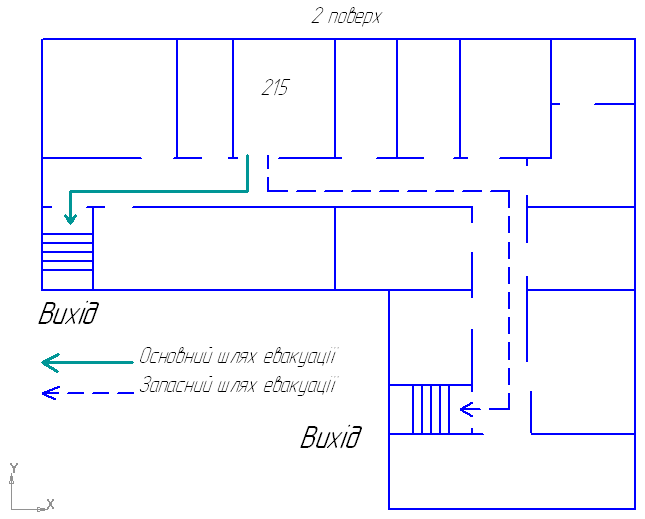
\includegraphics[scale=0.4]{lab_plan3}
\caption{План евакуації}\label{fig:lab_evac}
\end{figure}


\subsection{Висновок}
В роботі проаналізовано основні небезпечні чинники, можна відзначити, що при дотриманні правил безпеки і виробничої санітарії обладнання навігаційної системи не є пожежонебезпечним. Запропоновані світлодіодні світильники мають строк служби 50 тисяч годин, що значно краще ніж у люмінесцентних ламп, де строк рівний 10 - 20 тисяч годин, і крім того залежить від кількості переключень. З іншого боку світильники є економічнішими на 44.4 \% (світлодіодна лампа 20 +/- 1 Вт, люмінісцентна 36 +/-1Вт), більш ударостійкі, не містять токсичних речовин і не мають спеціальних вимог щодо утилізації. Ці лампи створюють оптимальні умови для зорової роботи інженера програміста, а порівняно не висока температура нагрівання підвищує рівень пожежної безпеки.

% \end{document}
